\documentclass{beamer}
\mode<presentation>
\usepackage{amsmath}
\usepackage{amssymb}
\usepackage{bm}
%\usepackage{advdate}
\usepackage{adjustbox}
\usepackage{subcaption}
%\usepackage{enumitem}
\usepackage{enumerate}
\usepackage{multicol}
\usepackage{mathtools}
\usepackage{listings}
\usepackage{url}
\def\UrlBreaks{\do\/\do-}
\usetheme{Boadilla}
\usecolortheme{lily}
\setbeamertemplate{footline}
{
  \leavevmode%
  \hbox{%
  \begin{beamercolorbox}[wd=\paperwidth,ht=2.25ex,dp=1ex,right]{author in head/foot}%
    \insertframenumber{} / \inserttotalframenumber\hspace*{2ex} 
  \end{beamercolorbox}}%
  \vskip0pt%
}
\setbeamertemplate{navigation symbols}{}

\providecommand{\nCr}[2]{\,^{#1}C_{#2}} % nCr
\providecommand{\nPr}[2]{\,^{#1}P_{#2}} % nPr
\providecommand{\mbf}{\mathbf}
\providecommand{\pr}[1]{\ensuremath{\Pr\left(#1\right)}}
\providecommand{\qfunc}[1]{\ensuremath{Q\left(#1\right)}}
\providecommand{\sbrak}[1]{\ensuremath{{}\left[#1\right]}}
\providecommand{\lsbrak}[1]{\ensuremath{{}\left[#1\right.}}
\providecommand{\rsbrak}[1]{\ensuremath{{}\left.#1\right]}}
\providecommand{\brak}[1]{\ensuremath{\left(#1\right)}}
\providecommand{\lbrak}[1]{\ensuremath{\left(#1\right.}}
\providecommand{\rbrak}[1]{\ensuremath{\left.#1\right)}}
\providecommand{\cbrak}[1]{\ensuremath{\left\{#1\right\}}}
\providecommand{\lcbrak}[1]{\ensuremath{\left\{#1\right.}}
\providecommand{\rcbrak}[1]{\ensuremath{\left.#1\right\}}}
\providecommand{\rank}{\text{rank}}
\theoremstyle{remark}
\newtheorem{rem}{Remark}
\newcommand{\sgn}{\mathop{\mathrm{sgn}}}
\providecommand{\abs}[1]{\left\vert#1\right\vert}
\providecommand{\res}[1]{\Res\displaylimits_{#1}} 
\providecommand{\norm}[1]{\lVert#1\rVert}
\providecommand{\mtx}[1]{\mathbf{#1}}
\providecommand{\mean}[1]{E\left[ #1 \right]}
\providecommand{\fourier}{\overset{\mathcal{F}}{ \rightleftharpoons}}
%\providecommand{\hilbert}{\overset{\mathcal{H}}{ \rightleftharpoons}}
\providecommand{\system}{\overset{\mathcal{H}}{ \longleftrightarrow}}
	%\newcomamand{\solution}[2]{\vec{Solution:}{#1}}
%\newcommand{\solution}{\noindent \vec{Solution: }}
\providecommand{\dec}[2]{\ensuremath{\overset{#1}{\underset{#2}{\gtrless}}}}
\newcommand{\myvec}[1]{\ensuremath{\begin{pmatrix}#1\end{pmatrix}}}
\newenvironment{amatrix}[1]{%
  \left(\begin{array}{@{}*{#1}{c}|c@{}}
}{%
  \end{array}\right)
}
\let\vec\mathbf

\lstset{
%language=C,
frame=single, 
breaklines=true,
columns=fullflexible
}

%\numberwithin{equation}{section}

\title{Matgeo-q.2.2.29}
\author{AI25BTECH11036-SNEHAMRUDULA}

\date{\today} 
\begin{document}

\begin{frame}
\titlepage
\end{frame}

\section*{Outline}


\begin{frame}
\frametitle{Question}
 Find the angle between the two planes $3x - 6y + 2z = 7$ and $2x + 2y - 2z = 5$.

\end{frame}
%
% --- FRAME 1 ---------------------------------------------------
\begin{frame}[t]{Solution}
\small
\textbf{Given:}\;
 The normal vectors of the planes are: \begin{align} \vec{n}_1 &= \myvec{3 \\ -6 \\ 2} \\ \vec{n}_2 &= \myvec{2 \\ 2 \\ -2} \end{align} The angle$\theta$ between the planes is given by: \begin{align} \cos \theta &= \frac{|\vec{n}_1^\top \vec{n}_2|}{\|\vec{n}_1\| \|\vec{n}_2\|} \end{align} Compute the dot product: \begin{align} \vec{n}_1^\top \vec{n}_2 &= (3)(2) + (-6)(2) + (2)(-2) = 6 - 12 - 4 = -10 \\ |\vec{n}_1^\top \vec{n}_2| &= 10 \end{align}
\end{frame}
 \begin{frame}
 Compute the magnitudes: \begin{align} \|\vec{n}_1\| &= \sqrt{3^2 + (-6)^2 + 2^2} = \sqrt{9 + 36 + 4} = \sqrt{49} = 7 \\ \|\vec{n}_2\| &= \sqrt{2^2 + 2^2 + (-2)^2} = \sqrt{4 + 4 + 4} = \sqrt{12} = 2\sqrt{3} \end{align} Thus, \begin{align} \cos \theta &= \frac{10}{7 \cdot 2\sqrt{3}} = \frac{5}{7\sqrt{3}} \\ \theta &= \cos^{-1} \left( \frac{5}{7\sqrt{3}} \right) \end{align} Therefore,the angle between the planes is:

\boxed{\cos^{-1} \left( \frac{5}{7\sqrt{3}} \right)}
\end{frame}
    \begin{frame}{Graphical Representation}

   \begin{figure}[h!]
\centering
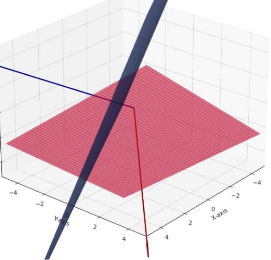
\includegraphics[width=0.7\linewidth]{fig.2.2.29.}

\end{figure}
\end{frame}
\end{document}


\end{document}